% Chapter Template

\chapter{A Work Sharing Framework} % Main chapter title

\label{Chapter3} % Change X to a consecutive number; for referencing this chapter elsewhere, use \ref{ChapterX}

\lhead{Chapter 3. \emph{Apache SparkSQL}} % Change X to a consecutive number; this is for the header on each page - perhaps a shortened title

%----------------------------------------------------------------------------------------
%	SECTION 1
%----------------------------------------------------------------------------------------

\section{Work Sharing}

In large data ware houses, many queries are usually submitted at the same time by multiple users. In the context of big data, a query would take long time to run. There are some data that would be used more frequently than the others, so we can avoid the redundant computations by sharing works among those queries and reduce the total amount of execution time. \\
The idea of work sharing originally comes from Multiple Query Optimization (MQO) \cite{sellis1988}. There are many works on traditional database systems \cite{cosar1993} \cite{bayir2007} \cite{georgios2012} \cite{stavros2005} and also on Hadoop MapReduce have been published. Olston et al. worked on a system called CoScan \cite{olston2011}, a system for sharing data and processing costs among multi-step MapReduce workflows which are executed in Hadoop. In Apache Pig, a number of work sharing optimizations \cite{pigmqo} have been used with the idea of MQO. The current state-of-the-art work in this field is MRShare\cite{nikiel2010} on Apache Hadoop. With the grouping technique, it provides the map input sharing to share scan of input files and map output sharing for saving cost of communication.\\
%----------------------------------------------------------------------------------------
%	SECTION 2
%----------------------------------------------------------------------------------------

\section{SparkSQL Server}
All the works above are only supported for Hadoop MapReduce and they are focused only on a part of work sharing, then they are hard to extend when users want to have new sharing techniques. To the best of our knowledges, there is no published work about Multi Query Optimization on Apache Spark. In our work, we present a new framework called SparkSQL Server, which is focused on work sharing among multiple queries.\\

SparkSQL Server supports queries written in SQL by using DataFrame API of SparkSQL or in produceral languague supported by SparkCore itself.\\

The framework does not only care about work sharing among multiple queries but also the scheduling mechanisms to associate with the sharing techniques or to fullfil the users' requirements.\\

The framework is generalized so it can support many types work sharing. All the modules of SparkSQL Server are easy to extend, this lets users and developers easily plug their own implementations into the framework.\\

\subsection{System Design}
The design of our framework aims at the generalization and extensibility so users and developers can easily plug their own implementations. Figure \ref{fig:sparksql-design} expresses the design of our system.\\
\begin{figure}
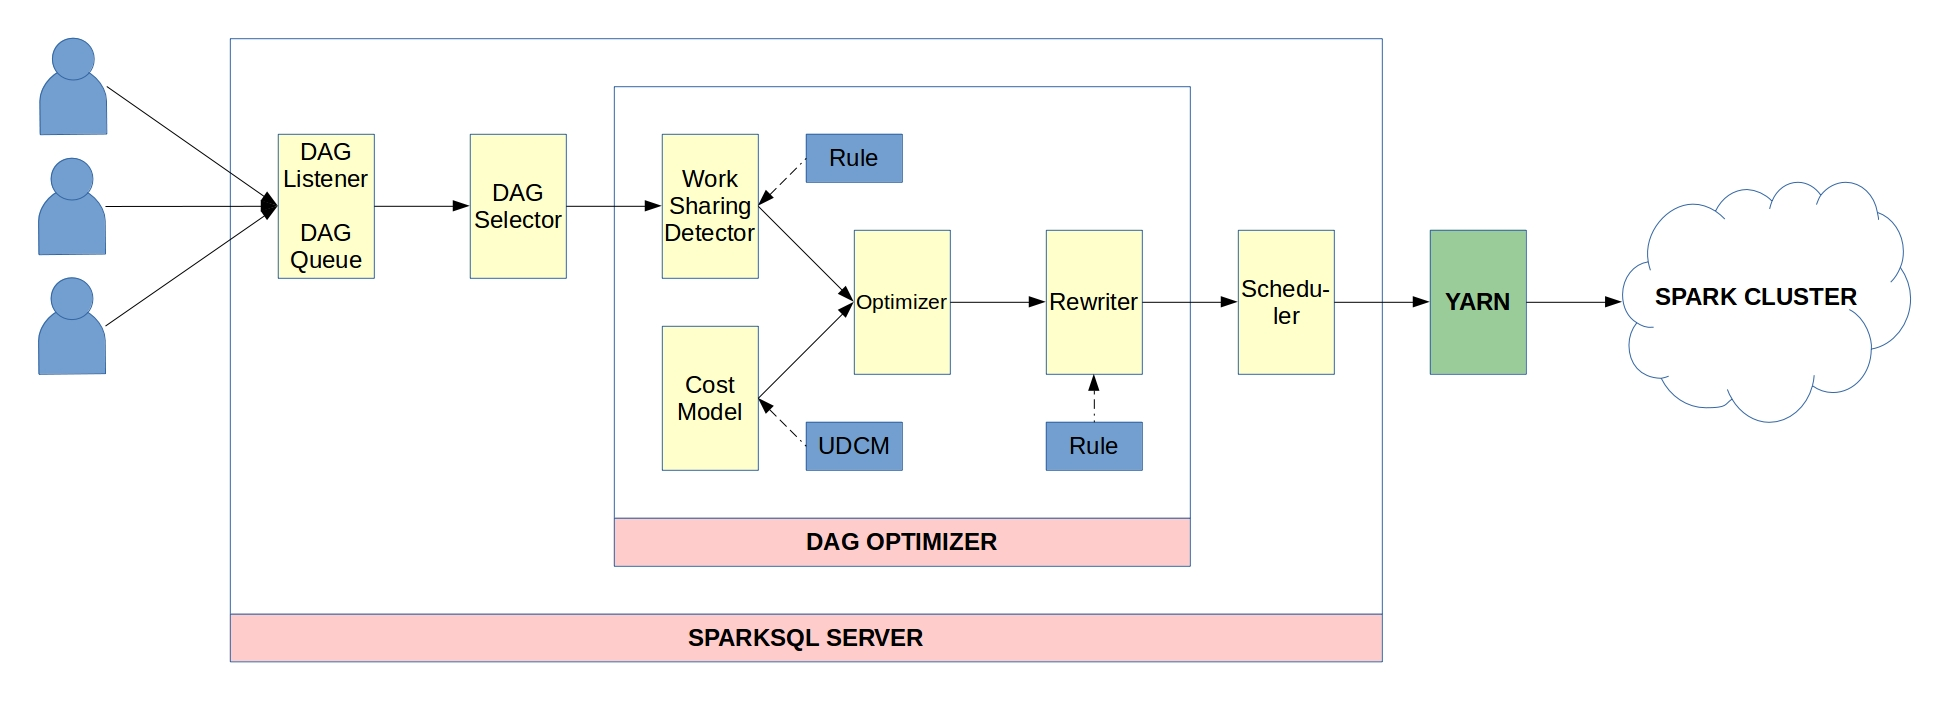
\includegraphics[width=\textwidth]{Figures/sparksql-server-design.jpg}
\label{fig:sparksql-design}
\caption{The design of SparkSQL Server}
\end{figure}

In overall, our framework has two sides: client side and server side.\\
\textbf{Client side} The client submits the query and needed information to SparkSQL Server so SparkSQL Server can reconstruct exactly the query happened at client side. The query can be written by using produceral operations in Spark or relational operations in SparkSQL or the combination of both types of operations.\\
\textbf{Server side}  The SparkSQL Server contains three main components:\\
\begin{itemize}
\item The Listeners, which are listened to client connections and communicate with them.
\item The DAG Optimizer are the hearts of our framework. All the detections, optimizations, and transformations happen here. The DAG Optimizer is composed of:
\begin{itemize}
\item WorkSharing Detector: this module detects the sharing opportunities among a batch of jobs which has just received from clients. The detector uses the rule-based mechanism to detect the sharable jobs. Users can easily write their own rules to detect sharable jobs with many types of sharing.
\item CostModel: it calculates the cost of each execution plan. Users provide their own cost model by the User-defined Cost Model.
\item Optimizer: it receives the input from the output of WorkSharing Detector and uses the CostModel to pick the best plan to execute.
\item Rewriter: the Rewriter transforms the original execution plans into the optimized execution plans and then submits them to the Schedulers. The transformation is also based on the rule-based mechanism. It is very easy to define a new rule to support another type of sharing.
\end{itemize} 
Again, all of these four modules are extendable so users can plug their owns into these modules.
\item The Schedulers, which are used to fulfill users' requirements and to associate with the sharing techniques. These Schedulers are aslo extendable so users can plug their own shechuling strategies.
\end{itemize}

\subsection{Implementations}
Similar to the above subsection, we present the implementations of our framework on both client side and server side. The order of the explaination is the same as the flow in figure \ref{fig:sparksql-design}.\\
\textbf{Client side} We will modify the spark-submit command so that it will not send the application to the cluster manager but to the SparkSQL Server, using this option:  --sparksql-server\\
Each client starts it own driver with its own SparkContext. Then, the client can generate its DAG, the DataFrame creation and send those information: DAG, DataFrame generation, SQL Query to the SparkSQL Server.\\
The client needs to send the jar file, because it contains all user defined functions, classes which are very important to reassemble the DAG at server side. It also needs to sends needed information so the SparkSQL Server can reconstruct the DAG and the query. Don’t forget that the query has already been optimized by Catalyst at the client side.\\
\textbf{Server side}
\begin{itemize}
\item \textbf{DAG Listener and DAG Queue} DAG Listener will accept the clients’ connections and receive DAGs, queries and other information they send. Then, it passes to the DAG Queue, the DAG Queue accepts the information the clients send at the FIFO order. In this component, the full DAG of each user will be built based on the initial DAG, the DataFrame creation information and the query. The DAG Queue has a window with fixed size, after reaching the size of the windows, DAG Queue will send a batch of DAGs (and queries also) into the next components. The window size right now is fixed as a constant, it will be changed when we take care of scheduling.
\item \textbf{DAG Selector} This component is something called a pre-scheduler, which will based on the constraint attached with each query to fulfill user’s requirements. For example: job submitted with a deadline. Right now, it just uses the simple FIFO strategy.
\item \textbf{Worksharing Detector} This component will detect which DAGs have the opportunity for worksharing, which DAGs haven’t. Remember that worksharing here is not only sharing scan, it can also have other variants such as sharing group-by or join. It works as rule-based mechanism to detect the worksharing opportunity. 
\item \textbf{Cost Model} It provides an interface so that users can plug their own cost model, which is called User defined cost model, into the system.
\item \textbf{Optimizer} With a bag from the output of the previous and a cost model associated with its sharing type, the Optimizer component will do the job: pick the plan with the lowest cost.
\item \textbf{Rewriter} This component has many families of rewrite. Each family will have many rewrite rules. It will generate a rewritten DAG which can be optimized, and use the rule that Optimizer picked to transform the original DAGs into the new ones..
\end{itemize}

\subsection{An Example on SparkSQL Server}

This section gives us an example of SparkSQL Server in action so we can understand how SparkSQL Server works clearly.
Three examples below are similar to the example in section 2.2.3 and we focus only on scan sharing in this example. The explaination has three parts for each components: Input, Output, and we relate them to the example.\\
\textbf{User1}

\begin{lstlisting}
case class Teacher(name: String, age: Integer)
val input = sc.textFile("hdfs://A.txt")
val people = input.map(_.split(",")).map(p => Teacher(p(0), p(1).trim.toInt))
val peopleDF = people.toDF()
peopleDF.registerTempTable("people")
val teacher = sqlContext.sql("SELECT name FROM people WHERE age <= 50")
val result = teacher.map(t => "Name: " + t(0)).collect.foreach(println)
\end{lstlisting}

\textbf{User2}

\begin{lstlisting}
case class Student(fullname: String, age: Integer)
val input = sc.textFile("hdfs://A.txt")
val people = input.map(_.split(",")).map(p => Student(p(0), p(1).trim.toInt))
val peopleDF = people.toDF()
peopleDF.registerTempTable("people")
val student = sqlContext.sql("SELECT name FROM people WHERE age >= 19")
val result = student.map(t => "Name: " + t(0)).collect.foreach(println)
\end{lstlisting}

\textbf{User3}

\begin{lstlisting}
case class Person(name: String, age: Integer)
val input = sc.textFile("hdfs://B.txt")
val people = input.map(_.split(",")).map(p => Persion(p(0), p(1).trim.toInt))
val peopleDF = people.toDF()
peopleDF.registerTempTable("people")
val adults = sqlContext.sql("SELECT name FROM people WHERE age >= 25")
val result = adults.map(t => "Name: " + t(0)).collect.foreach(println)
\end{lstlisting}

\textbf{Client Side}
\begin{itemize}
\item Input: Users’ applications (jar files)
\item Output: Jarfile, DAGs, DataFrame creation information, SQL queries are sent to SparkSQL Server. In those example, we have DAG1, DAG2, DAG3.
\end{itemize}

\textbf{Server Side}\\
\textbf{DAG Listener and DAG Queue}
\begin{itemize}
\item Input: DAGs and queries from clients
\item Output: Batch of DAGs, queries, DataFrame creation information after reaching the window size of DAG Queue
\item In the example, let assume the window size of DAG Queue is 3, so the output will be DAG1, DAG2, DAG3. If there is user4 submits the job, it will be packed with another two jobs.
\end{itemize}

\textbf{DAG Selector}
\begin{itemize}
\item Input: Batch of DAGs
\item Output: Batch of DAGs based on scheduling strategies (FIFO at the moment).
\item In the example, the input and the output is the same as we use FIFO strategy.
\end{itemize}

\textbf{Worksharing Detector}
\begin{itemize}
\item Input: Batch of DAGs
\item Output: Bags of DAGs which are labeled each type of sharing (sharing scan, sharing groupby…) or "no sharing".
\item In the example, we got two Bags: DAGBag1: {DAG1, DAG2} with the label: “scan sharing”; DAGBag2: {DAG3} with the label: "no sharing".
\end{itemize}

\textbf{Cost Model}
\begin{itemize}
\item Input: a DAG and its metadata to compute the cost
\item Output: costs belong to DAGs
\item In the example, we use the MRShare Cost Model so it returns a bag of DAG which can be merged together which is DAGBag1: {DAG1, DAG2}.
\end{itemize}

\textbf{Optimizer}
\begin{itemize}
\item Input: Bags of sharable DAGs, a Cost Model associated to the sharing type of each bag.
\item Output: Bags of optimized DAGs.
\item In the example, we got DAGBag1: {DAG1, DAG2}, DAGBag2: {DAG3}
\end{itemize}

\textbf{Rewriter}
\begin{itemize}
\item Input: Optimized Bags of DAGs
\item Output: Rewritten Bags of DAGs
\item In the example, since MRShare uses the simultaneous pipeline technique to merge jobs, we got DAGBag1: {DAG12}, DAGBag2: {DAG3}
\end{itemize}

\textbf{PostScheduler}
\begin{itemize}
\item Input: Rewritten Bags of DAGs
\item In the example, we got 2 Bags of DAGs. Since the execution order does not affect these jobs or in other way, they are independent on each other, so we just use FIFO strategy to submit to the cluster.
\end{itemize}

The example is only for scan sharing and just to show the dataflow of SparkSQL Server but the system is generalized and extensible so other sharing techniques can be embedded into the system.